\documentclass[compress]{thesisbeamer}
\useoutertheme[subsection=false]{miniframes}

\title{A Gazebo Simulator for Continuum Parallel Robots}
\author[Gotelli Andrea]{Author Gotelli Andrea\newline ~ \newline \normalsize{Advisors: Duh, Dih, Dah}}
\date{22/02/2021}

\bibliography{../biblio}

% video will work on Linux (with Okular) or OS X, for other OS's or viewers find your own way to do it
%\videoOSX	% for OS X 
%\videoOFF
\begin{document}

\MakeTitleNoFoot

    
   	\section{Introduction}
        \subsection{Subsection1}
        \begin{frame}
            \begin{columns}
			\column{0.5\textwidth}
			\begin{itemize}%[<+->]
  				\item Serial robots
  				\begin{itemize}%[<.->]
   					\item Simpler and more used
   					\item Limited by precision and inertia
  				\end{itemize}\vfill
  				\item Parallel robots
  				\begin{itemize}%[<.->]
   					\item Less inertia, high velocities
   					\item More joints involved
  				\end{itemize}\vfill
 			\end{itemize}
			\vspace{2cm}
			\column{0.5\textwidth}
			\begin{figure}[h]
				\centering
				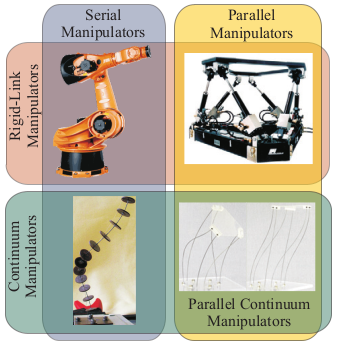
\includegraphics[width=\textwidth]{images/serial_parall_robots}
				\caption{Different robot architectures}
			\end{figure}
			\end{columns}
		\end{frame}

        \subsection{Subsection2}
        \begin{frame}
			\begin{columns}
			\column{0.5\textwidth}
			\begin{itemize}%[<+->]
  				\item Continuum parallel robots 
  				\begin{itemize}%[<.->]
   					\item May anhance safety
   					\item Cheaper components 
   					\item Possible to miniturize
  				\end{itemize}
  				\item Model and stability problems
  				\begin{itemize}%[<.->]
   					\item More unstable configurations
   					\item Another drawback
   					\item Not analytical solution
  				\end{itemize}
 			\end{itemize}
			\vspace{2cm}
			\column{0.5\textwidth}
			\begin{figure}[h]
				\centering
				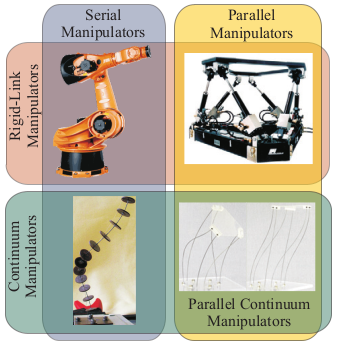
\includegraphics[width=\textwidth]{images/serial_parall_robots}
				\caption{Different robot architectures.}
			\end{figure}
			\end{columns}
		\end{frame}
		
		\subsection{Subsection3}
        \begin{frame}
        	\frametitle{CPR simulator}
			\begin{itemize}%[<+->]
  				\item General simulator 
  				\begin{itemize}%[<.->]
   					\item Gazebo
   					\item Different robots
  				\end{itemize}
  				\item Solve the modelling
  				\begin{itemize}%[<.->]
   					\item Rod statics
   					\item Robot assembly
   					\item Visual interface
   					\item Robot dynamics
  				\end{itemize}
 			\end{itemize}
		\end{frame}


        \section{Methods}
        	\subsection{Subsection1}
        	\begin{frame}
        		\frametitle{Geometric modelling}
				\begin{columns}
				\column{0.5\textwidth}
				\begin{itemize}%[<+->]
  					\item Rod as 1D body 
  					\item Function of the arc-lenght
  					\begin{itemize}%[<.->]
   						\item Centerline position
   						\item Cross-section orientation
  					\end{itemize}
 				\end{itemize}
				\vspace{2cm}
				\column{0.5\textwidth}
				\begin{figure}[h]
					\centering
					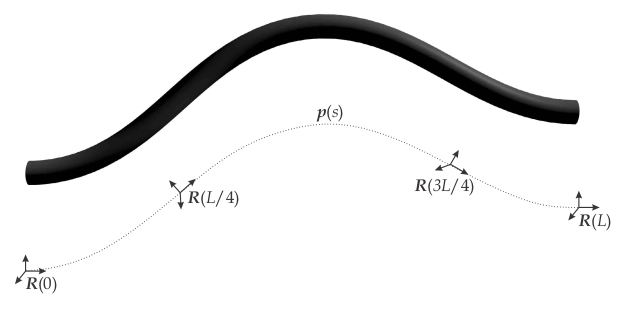
\includegraphics[width=\textwidth]{images/rod_geometry}
					\caption{Rod geometric modelling}
				\end{figure}
				\end{columns}
			\end{frame}

        \subsection{Subsection2}
        \begin{frame}
        	\frametitle{Equilibrium Equations}
			\begin{columns}
			\column{0.5\textwidth}
			\begin{itemize}%[<+->]
  				\item Equilibrium consideration
  				\begin{itemize}%[<.->]
   					\item Distributed forces/moments
   					\item Internal forces/moments
  				\end{itemize}
 			\end{itemize}
			\vspace{2cm}
			\column{0.5\textwidth}
			\begin{figure}[h]
				\centering
				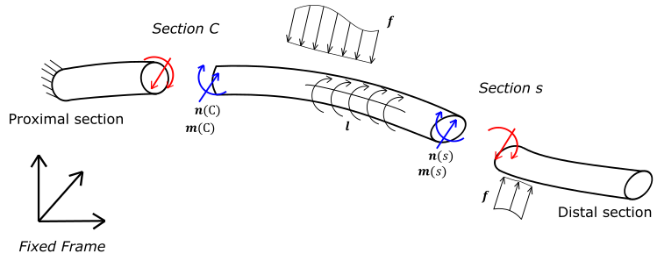
\includegraphics[width=\textwidth]{images/equilibrium}
				\caption{Sections of the beam considered for the static equilibrium.}
			\end{figure}
			\end{columns}
		\end{frame}

        \subsection{Subsection3}
        \begin{frame}
			\begin{columns}
			\column{0.5\textwidth}
			\begin{itemize}%[<+->]
  				\item Boundary value problem
  				\item Constraints at the platform
  				\begin{itemize}%[<.->]
   					\item External wrench
   					\item Joints and geometry
  				\end{itemize}
  				\item Constraints at the base 
  				\begin{itemize}%[<.->]
   					\item Actuations
   					\item Joints and geometry 
  				\end{itemize}
 			\end{itemize}
			\vspace{2cm}
			\column{0.5\textwidth}
			\begin{figure}[h]
				\centering
				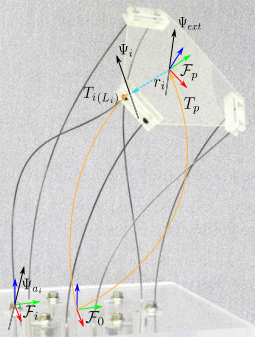
\includegraphics[width=\textwidth]{images/BVP}
				\caption{Sections of the beam considered for the static equilibrium.}
			\end{figure}
			\end{columns}
		\end{frame}
		
		\subsection{Subsection4}
        \begin{frame}
			\begin{columns}
			\column{0.5\textwidth}
			\begin{itemize}%[<+->]
  				\item Shooting Method
  				\begin{itemize}
  					\item ODE system in statics
  					\item Needs an intial guess
  					\item Recursive
  				\end{itemize}
  				\item Evaluation on a cost function
  				\item Sensitive to initial conditions
 			\end{itemize}
			\vspace{2cm}
			\column{0.5\textwidth}
			\begin{figure}[h]
				\centering
				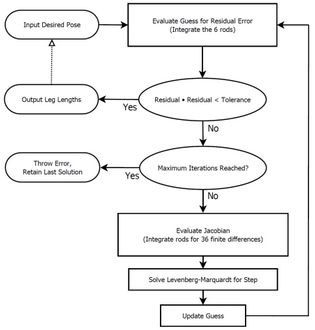
\includegraphics[width=\textwidth]{images/sequence}
				\caption{Recursive process for Shooting method.}
			\end{figure}
			\end{columns}
		\end{frame}
		
		\subsection{Subsection5}
        \begin{frame}
			\begin{itemize}%[<+->]
  				\item Shooting Method
  				\begin{itemize}
  					\item PDE system in dynamics
  					\item Numerical discretization
  					\item Recursive
  				\end{itemize}
  				\item Evaluation on a cost function
  				\item Sensitive to initial conditions
 			\end{itemize}
		\end{frame}
		
		\subsection{Subsection6}
        \begin{frame}
			\begin{itemize}%[<+->]
  				\item Strain Approach
  				\begin{itemize}
  					\item Intro here
  				\end{itemize}
 			\end{itemize}
		\end{frame}
		
		\subsection{Subsection7}
        \begin{frame}
			\begin{itemize}%[<+->]
  				\item Strain Approach
  				\begin{itemize}
  					\item Details here
  				\end{itemize}
 			\end{itemize}
		\end{frame}

        \section{Conclusions}
        \begin{frame}
            \frametitle{Frame3}
        \end{frame}

        \frame{}

\end{document}
